% Slide 7 -- SAM segmentation + propagation
\begin{frame}{Stage 1: SAM segmentation + bidirectional propagation}
  \begin{columns}[T]
    \begin{column}{0.55\textwidth}
      \begin{block}{Foundation-model segmentation}
        \footnotesize
        \begin{itemize}
          \item \alert{SAM (ViT-B)} as a frozen segmenter --- no training, no labels.
          \item One seed slice (click \emph{or} automatic point at $0.40 W, 0.40 H$).
          \item Morphological refinement: small-object removal, hole filling, opening/closing.
        \end{itemize}
      \end{block}

      \begin{block}{Bidirectional propagation, dynamic Dice}
        \footnotesize Centroid of slice $i$ $\to$ positive prompt for $i\!\pm\!1$. \alert{Adaptive threshold}:
        \[
          \tau_i = 0.45 + 0.25 \cdot |i - i_\text{seed}| / \Delta_\text{max}
        \]
        Strict near the seed, permissive at extremes. \alert{Negative-prompt} fallback for failures.
      \end{block}
    \end{column}
    \begin{column}{0.45\textwidth}
      \centering
      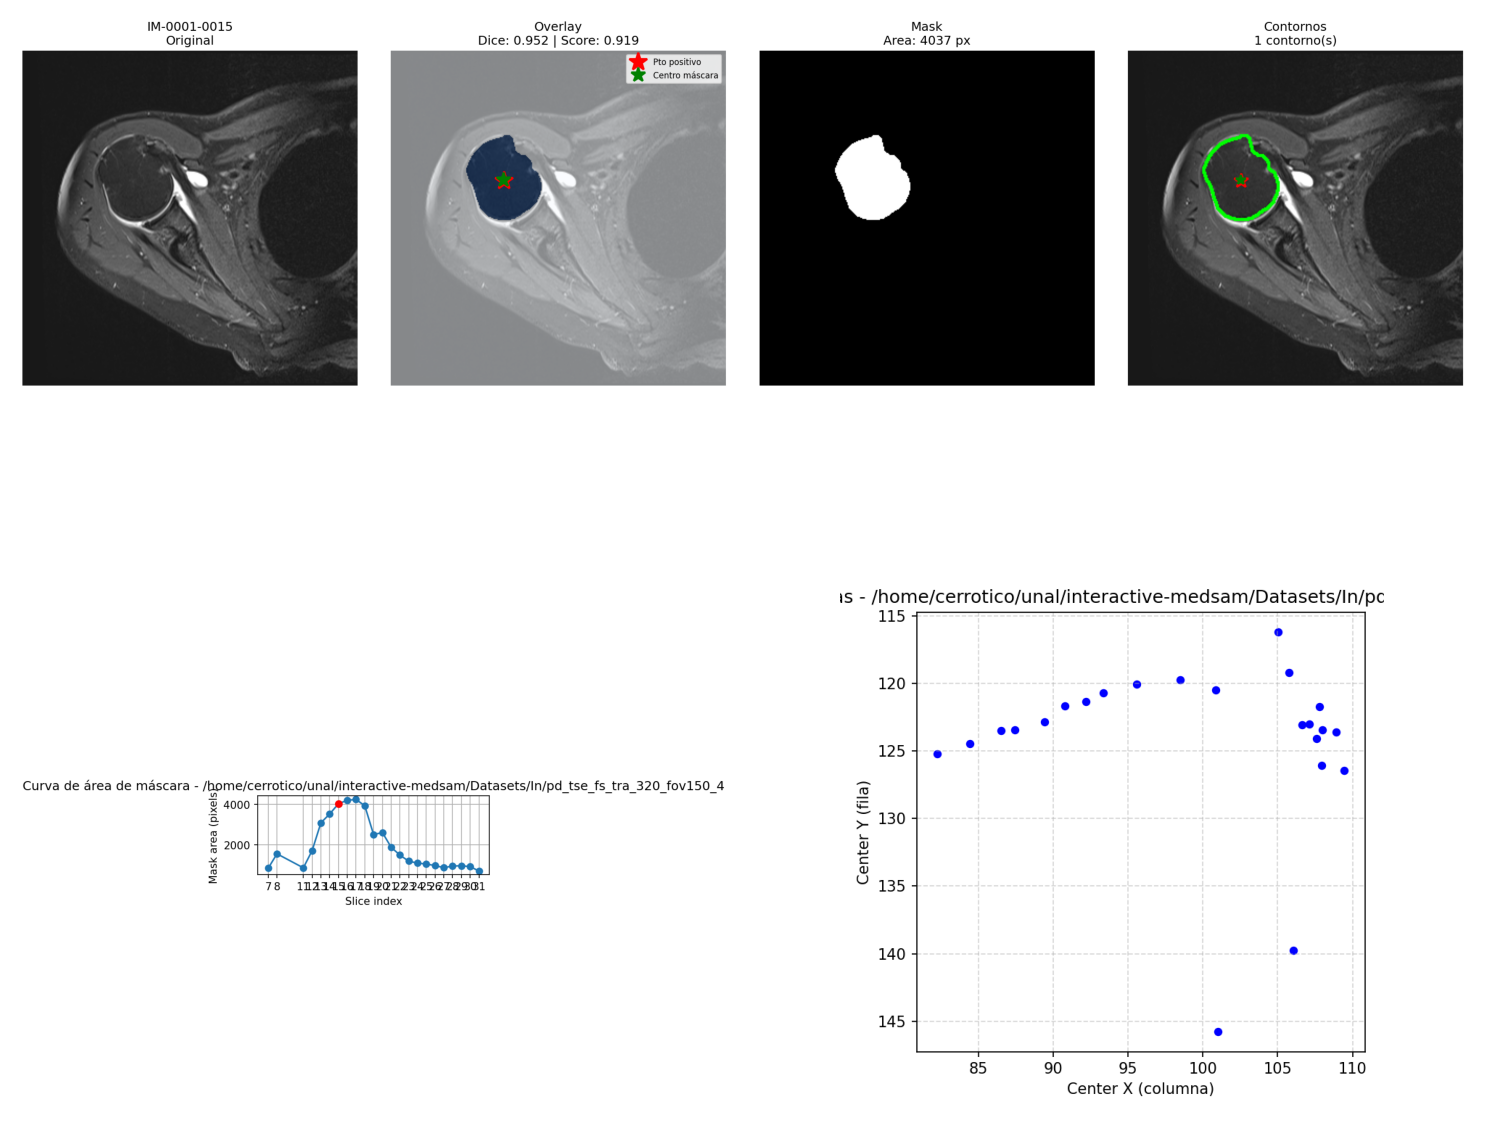
\includegraphics[width=\linewidth]{figures/seg_example.png}
      \\[0.3em]
      {\footnotesize Per-slice segmentation overlay.\\ Green = mask boundary;\\ red dot = positive prompt centroid.}
    \end{column}
  \end{columns}
\end{frame}
